%!TEX program = tectonic
\documentclass[11pt,letterpaper,oneside]{report}
\usepackage{../anahuac}
\materia{Inteligencia Artificial Aplicada}
\sesion{6}{Modelos de lenguaje con un mini GPT}
\subtitulo{De los subtítulos de \emph{Teresa} a un transformer que escribe como telenovela}
\graphicspath{{figuras/}}
% GENERADO por scripts/figuras_minigpt.py a partir de data/processed/minigpt_teresa.json
\newcommand{\mgCorpusMB}{2.52}
\newcommand{\mgCapitulos}{152}
\newcommand{\mgCapitulosVal}{15}
\newcommand{\mgTokensTrain}{663\,225}
\newcommand{\mgTokensVal}{66\,534}
\newcommand{\mgCharsToken}{3.37}
\newcommand{\mgParametros}{12\,281\,856}
\newcommand{\mgParametrosM}{12.3}
\newcommand{\mgPasos}{4\,000}
\newcommand{\mgMejorPaso}{2\,000}
\newcommand{\mgMejorVal}{3.56}
\newcommand{\mgMejorPPL}{35.0}
\newcommand{\mgMinutos}{10}
\newcommand{\mgVRAM}{1.3}
\newcommand{\mgVocab}{4000}
\newcommand{\mgLnV}{8.29}
\newcommand{\mgEpocas}{49}
\newcommand{\mgEpocasMejor}{25}
\newcommand{\mgValFinal}{3.69}
\newcommand{\mgTrainFinal}{1.67}
\newcommand{\mgDescartado}{99}

\newcommand{\esp}{\textcolor{anahuac}{\_}}
\newcommand{\tok}[1]{\colorbox{naranjabg}{\strut\ttfamily\small #1}}
\begin{document}
\portada
\tableofcontents
\setcounter{chapter}{5}
\chapter{Modelos de lenguaje con un mini GPT}

\section{Un modelo que adivina la siguiente palabra}

Imagina que estás frente al televisor, es 2010 y en pantalla Arturo de la Barrera mira fijamente a Teresa Chávez. Ella abre la boca y dice: \emph{``Arturo, yo te\ldots''}. Si has visto suficientes telenovelas, tu cerebro ya completó la frase. Quizá \emph{``amo''}, quizá \emph{``odio''}, quizá \emph{``juro que me las vas a pagar''}. Ese acto de anticipar lo que sigue a partir de lo que ya se dijo es, literalmente, lo único que hace un modelo de lenguaje como GPT.

En esta sesión vamos a construir uno desde cero. Le daremos como único material de estudio los diálogos de \emph{Teresa} (Televisa, 2010), una telenovela sobre una joven brillante y ambiciosa que quiere salir de la vecindad a cualquier costo. El modelo nunca ha visto español: empieza adivinando al azar y, después de unos minutos de entrenamiento en una tarjeta gráfica, termina escribiendo reclamos, juramentos y declaraciones de amor con el tono inconfundible del género.

\subsection{La factorización que lo hace posible}

Un texto es una secuencia de símbolos $x_1, x_2, \dots, x_T$. La regla de la cadena de la probabilidad dice que la probabilidad conjunta de toda la secuencia se puede escribir como un producto de probabilidades condicionales:
\begin{equation}\label{eq:cadena}
  p(x_1, x_2, \dots, x_T) = \prod_{t=1}^{T} p(x_t \mid x_1, \dots, x_{t-1}).
\end{equation}
Esta identidad es exacta y no supone nada. Un \textbf{modelo de lenguaje autorregresivo} aproxima cada factor con una red neuronal de parámetros $\theta$, que recibe el contexto $x_{<t}$ y devuelve una distribución sobre el siguiente símbolo:
\[
  p_\theta(x_t \mid x_{<t}).
\]
Si la red aprende bien esos factores, sirve para dos cosas. La primera es \emph{evaluar}: asignar una probabilidad a un texto, lo cual permite medir qué tan bien ``entiende'' el modelo un capítulo que nunca vio. La segunda es \emph{generar}: tomar un comienzo, muestrear el siguiente símbolo, agregarlo al contexto y repetir.

\begin{intuicion}
Un modelo de lenguaje es un autocompletado con memoria larga. El autocompletado del teléfono mira dos o tres palabras; un transformer mira cientos de símbolos a la vez y decide, para cada uno, cuánto pesa en la predicción.
\end{intuicion}

\subsection{El corpus de esta sesión}

Los capítulos de \emph{Teresa} están en YouTube, publicados por canales de Televisa y de aficionados. El script \texttt{scripts/descargar\_teresa.py} busca capítulos y escenas, descarga solo los subtítulos en español (casi todos generados por el reconocimiento automático de voz) y los limpia: elimina marcas de tiempo, etiquetas y anotaciones como \texttt{[Música]}, quita las repeticiones que produce el subtítulo automático y descarta las escenas sueltas que repiten un capítulo ya incluido. Con esto se reunieron \mgCapitulos{} videos y \mgCorpusMB{}~MB de diálogo. Un fragmento real del corpus:

\begin{lstlisting}[language={},numbers=none,basicstyle=\ttfamily\footnotesize]
Eres peor de lo que pensaba, Teresa.
Fuera de aquí.
Fuera de aquí. No quiero verte más.
Arturo, por favor, piénsalo.
Tú y yo aún estamos a tiempo de ser
felices. No, Teresa, tuviste muchas
oportunidades y todas las
desperdiciaste.
\end{lstlisting}

El texto tiene errores de transcripción y renglones cortados a la mitad de una frase. Lo dejamos así a propósito: un modelo de lenguaje aprende la distribución de su corpus con todo y sus defectos, y conviene verlo con nuestros propios ojos.

\begin{nota}[Derechos]
Los diálogos pertenecen a Televisa. El corpus se usa solo para entrenar un modelo didáctico, vive en una carpeta excluida del repositorio (\texttt{data/raw/teresa/}) y no se redistribuye.
\end{nota}

\subsection{El plan}

El camino de esta sesión sigue el recorrido de un símbolo por dentro del modelo, mostrado en la figura~\ref{fig:panorama}: el texto se parte en \emph{tokens} (sección~\ref{sec:bpe}), cada token se vuelve un vector (sección~\ref{sec:emb}), los vectores conversan entre sí mediante atención (secciones~\ref{sec:atencion} y \ref{sec:multi}) dentro de bloques que se apilan (sección~\ref{sec:bloque}), y al final una capa lineal produce una puntuación para cada token posible. Después veremos cómo se entrena (sección~\ref{sec:entrenamiento}) y cómo se genera texto (sección~\ref{sec:generacion}).

\begin{figure}[H]
\centering
\begin{tikzpicture}[
  caja/.style={draw=pizarra, rounded corners=3pt, minimum height=8mm, minimum width=24mm, font=\sffamily\small, align=center, fill=white},
  naranja/.style={caja, fill=naranjabg, draw=anahuac},
  flecha/.style={-Stealth, thick, pizarra}]
\node[font=\ttfamily\small] (txt) at (0,0) {«yo te amo»};
\node[caja, right=6mm of txt] (tok) {Tokenizador\\BPE};
\node[caja, right=6mm of tok] (emb) {Embeddings\\token + posición};
\node[naranja, right=6mm of emb, minimum height=14mm] (blq) {$N$ bloques\\transformer};
\node[caja, right=6mm of blq] (out) {Lineal +\\softmax};
\node[font=\sffamily\small, below=7mm of out, align=center] (p) {$p_\theta(\,\cdot \mid \text{contexto})$};
\draw[flecha] (txt) -- (tok);
\draw[flecha] (tok) -- node[above, font=\scriptsize]{ids} (emb);
\draw[flecha] (emb) -- (blq);
\draw[flecha] (blq) -- (out);
\draw[flecha] (out) -- (p);
\end{tikzpicture}
\caption{Recorrido completo de un modelo de lenguaje tipo GPT. Todo lo que está entre el tokenizador y la salida se aprende con descenso de gradiente.}
\label{fig:panorama}
\end{figure}

\begin{ejercicio}
\begin{enumerate}[label=\alph*)]
  \item Escribe la factorización~\eqref{eq:cadena} para la frase de tres palabras ``te amo Teresa''. ¿Cuántas distribuciones condicionales distintas tiene que aprender el modelo para esa frase?
  \item Un modelo que ignora el contexto y siempre usa la frecuencia global de cada palabra se llama \emph{modelo unigrama}. Escribe su factorización. ¿Qué frase le asignaría la misma probabilidad que ``te amo Teresa''?
\end{enumerate}
\end{ejercicio}

% ===========================================================================
\section{Tokenización: partir el texto en piezas}\label{sec:bpe}

La red neuronal solo sabe multiplicar números, así que el primer paso es convertir el texto en una secuencia de enteros. La pregunta es qué unidad usar.

\begin{itemize}
  \item \textbf{Palabras completas.} El corpus de \emph{Teresa} tiene decenas de miles de palabras distintas y la mayoría aparece una o dos veces. El modelo tendría muy pocos ejemplos de cada una, y una palabra nueva (un nombre, un error de transcripción) no tendría representación.
  \item \textbf{Caracteres.} El vocabulario es pequeño (un centenar de símbolos), pero las secuencias se alargan tres o cuatro veces. Como el costo de la atención crece con el cuadrado de la longitud, esto encarece cada paso.
  \item \textbf{Subpalabras.} Un punto intermedio: las palabras frecuentes son un solo token y las raras se arman con pedazos frecuentes. Es lo que usan todos los modelos modernos.
\end{itemize}

\subsection{Byte-Pair Encoding}

\begin{definicion}[BPE]
Dado un corpus y un tamaño de vocabulario objetivo $V$, el algoritmo \emph{Byte-Pair Encoding} (Sennrich, Haddow y Birch, 2016) construye el vocabulario así:
\begin{enumerate}
  \item Inicia con los caracteres del corpus. Cada palabra se representa como una secuencia de caracteres y el espacio que la precede se marca con un símbolo especial, que aquí escribimos \esp.
  \item Cuenta, ponderando por la frecuencia de cada palabra, cuántas veces aparece cada par de símbolos adyacentes.
  \item Fusiona el par más frecuente en un símbolo nuevo y guarda la regla de fusión.
  \item Repite los pasos 2 y 3 hasta que el vocabulario tenga $V$ símbolos.
\end{enumerate}
Para tokenizar un texto nuevo se aplican las reglas de fusión en el mismo orden en que se aprendieron.
\end{definicion}

\begin{ejemplo}[BPE a mano con palabras de \emph{Teresa}]
Supongamos un corpus diminuto con cuatro palabras y estas frecuencias: \emph{es} (6 veces), \emph{eres} (5), \emph{teresa} (3) y \emph{ser} (2). Al inicio cada palabra es su secuencia de caracteres:
\[
\text{\esp\,e\,s}\ (6),\qquad \text{\esp\,e\,r\,e\,s}\ (5),\qquad \text{\esp\,t\,e\,r\,e\,s\,a}\ (3),\qquad \text{\esp\,s\,e\,r}\ (2).
\]
\textbf{Ronda 1.} Contamos pares. El par \texttt{e s} aparece en \emph{es}, \emph{eres} y \emph{teresa}: $6+5+3 = 14$ veces. El par \texttt{\esp{} e} suma $6+5 = 11$; \texttt{e r} suma $5+3+2 = 10$; \texttt{r e} suma $5+3 = 8$; los demás valen 3 o 2. Gana \texttt{e s} $\to$ \texttt{es}.

\textbf{Ronda 2.} Ahora las palabras son \esp\,es, \esp\,e\,r\,es, \esp\,t\,e\,r\,es\,a y \esp\,s\,e\,r. El par \texttt{e r} vale $5+3+2 = 10$, \texttt{r es} vale 8 y \texttt{\esp{} es} vale 6. Gana \texttt{e r} $\to$ \texttt{er}.

\textbf{Ronda 3.} El par \texttt{er es} aparece en \emph{eres} y \emph{teresa}: $5+3 = 8$. Gana y crea \texttt{eres}.

\textbf{Rondas 4 y 5.} Se fusionan \texttt{\esp{} es} (6) y \texttt{\esp{} eres} (5), que ya son palabras completas con su espacio inicial.

Las reglas aprendidas, en orden, son: \texttt{e+s}, \texttt{e+r}, \texttt{er+es}, \texttt{\esp+es}, \texttt{\esp+eres}. Para tokenizar la palabra nueva \emph{teresa} partimos de \esp\,t\,e\,r\,e\,s\,a y aplicamos las reglas en orden:
\[
\text{\esp\,t\,e\,r\,e\,s\,a} \xrightarrow{\ e+s\ } \text{\esp\,t\,e\,r\,es\,a} \xrightarrow{\ e+r\ } \text{\esp\,t\,er\,es\,a} \xrightarrow{\ er+es\ } \text{\esp\,t\,eres\,a}.
\]
Resultado: cuatro tokens, \tok{\esp}\,\tok{t}\,\tok{eres}\,\tok{a}. Con un corpus real, el nombre de la protagonista aparece miles de veces y termina siendo un solo token.
\end{ejemplo}

\begin{figure}[H]
\centering
\begin{tikzpicture}[
  c/.style={draw=azuldef, fill=azuldefbg, minimum height=6mm, minimum width=7mm, font=\ttfamily\small, inner sep=2pt, rounded corners=1pt},
  n/.style={c, draw=anahuac, fill=naranjabg},
  et/.style={font=\scriptsize\sffamily, text=gray, anchor=east}]
\foreach \s [count=\i] in {\esp,t,e,r,e,s,a} \node[c] (a\i) at (\i*0.85,0) {\s};
\node[et] at (0.3,0) {inicio};
\foreach \s [count=\i] in {\esp,t,e,r} \node[c] (b\i) at (\i*0.85,-1) {\s};
\node[n, minimum width=12mm] (b5) at (5.42,-1) {es};
\node[c] (b6) at (6.4,-1) {a};
\node[et] at (0.3,-1) {e+s};
\node[c] (c1) at (0.85,-2) {\esp}; \node[c] (c2) at (1.7,-2) {t};
\node[n, minimum width=12mm] (c3) at (2.85,-2) {er};
\node[c, minimum width=12mm] (c4) at (4.1,-2) {es}; \node[c] (c5) at (5.1,-2) {a};
\node[et] at (0.3,-2) {e+r};
\node[c] (d1) at (0.85,-3) {\esp}; \node[c] (d2) at (1.7,-3) {t};
\node[n, minimum width=20mm] (d3) at (3.3,-3) {eres}; \node[c] (d4) at (4.75,-3) {a};
\node[et] at (0.3,-3) {er+es};
\draw[-Stealth, anahuac, thick] (a5.south) -- (b5.north); \draw[-Stealth, anahuac, thick] (a6.south) -- (b5.north);
\draw[-Stealth, anahuac, thick] (b3.south) -- (c3.north); \draw[-Stealth, anahuac, thick] (b4.south) -- (c3.north);
\draw[-Stealth, anahuac, thick] (c3.south) -- (d3.north); \draw[-Stealth, anahuac, thick] (c4.south) -- (d3.north);
\end{tikzpicture}
\caption{Traza de las fusiones BPE del ejemplo para la palabra \emph{teresa}. En naranja, el símbolo recién creado en cada ronda.}
\label{fig:bpe}
\end{figure}

\subsection{SentencePiece y el vocabulario real}

En la práctica no programamos BPE a mano sobre millones de caracteres. Usamos \textbf{SentencePiece} (Kudo y Richardson, 2018), que implementa el mismo algoritmo de forma eficiente, trata el espacio como un carácter más (por eso aparece el símbolo \esp{} al inicio de muchas piezas) y permite reconstruir el texto original sin ambigüedad. Entrenamos un vocabulario de $V = \mgVocab$ piezas sobre el corpus completo. Con él, cada token equivale en promedio a \mgCharsToken{} caracteres, y el corpus se convierte en \mgTokensTrain{} tokens de entrenamiento y \mgTokensVal{} de validación.

Algunas frases reales pasadas por el tokenizador entrenado:
% GENERADO por scripts/figuras_minigpt.py
\begin{center}\small
\begin{tabular}{@{}p{0.34\textwidth}p{0.6\textwidth}@{}}
\toprule
Frase & Piezas del tokenizador entrenado \\
\midrule
\emph{Teresa, eres una ambiciosa} (7 tokens) & \tok{\esp{}Teresa}\,\tok{,}\,\tok{\esp{}eres}\,\tok{\esp{}una}\,\tok{\esp{}ambi}\,\tok{ci}\,\tok{osa} \\[2pt]
\emph{yo nunca me voy a casar contigo} (7 tokens) & \tok{\esp{}yo}\,\tok{\esp{}nunca}\,\tok{\esp{}me}\,\tok{\esp{}voy}\,\tok{\esp{}a}\,\tok{\esp{}casar}\,\tok{\esp{}contigo} \\[2pt]
\emph{Arturo de la Barrera} (4 tokens) & \tok{\esp{}Arturo}\,\tok{\esp{}de}\,\tok{\esp{}la}\,\tok{\esp{}Barrera} \\[2pt]
\emph{¿por qué me haces esto?} (7 tokens) & \tok{\esp{}¿}\,\tok{por}\,\tok{\esp{}qué}\,\tok{\esp{}me}\,\tok{\esp{}haces}\,\tok{\esp{}esto}\,\tok{?} \\[2pt]
\emph{la vecindad} (2 tokens) & \tok{\esp{}la}\,\tok{\esp{}vecindad} \\[2pt]
\bottomrule
\end{tabular}
\end{center}


\begin{nota}
Además de las piezas aprendidas, el vocabulario reserva símbolos especiales: \texttt{<unk>} para lo desconocido, \texttt{<s>} y \texttt{</s>} para inicio y fin, y en nuestro caso \texttt{<nl>} para el salto de línea entre renglones de subtítulo. Así el modelo aprende también dónde cortar.
\end{nota}

\begin{ejercicio}
\begin{enumerate}[label=\alph*)]
  \item Con las cinco reglas del ejemplo, tokeniza \emph{seres} y \emph{mesera}. ¿Cuántos tokens produce cada una?
  \item Agrega al corpus del ejemplo la palabra \emph{teresa} con frecuencia 10 y repite las tres primeras rondas. ¿Cambia el orden de las fusiones?
  \item Si el vocabulario tiene $V$ piezas y el texto tiene $N$ caracteres, explica por qué al aumentar $V$ disminuye el número de tokens pero crece la matriz de embeddings. ¿Qué dos costos se están equilibrando?
\end{enumerate}
\end{ejercicio}

% ===========================================================================
\section{De tokens a vectores: embeddings}\label{sec:emb}

Cada token es ahora un entero entre $0$ y $V-1$. La red lo traduce a un vector de dimensión $d$ consultando una tabla:

\begin{definicion}[Embedding de token]
Una \emph{tabla de embeddings} es una matriz de parámetros $W_E \in \R^{V\times d}$. El token con índice $i$ se representa con la fila $W_E[i] \in \R^d$. Equivale a multiplicar un vector \emph{one-hot} $e_i \in \R^V$ por la matriz: $e_i^\top W_E = W_E[i]$.
\end{definicion}

En nuestro modelo $d = 384$, así que la tabla tiene $\mgVocab \times 384$ números que al inicio son aleatorios y que el entrenamiento acomoda de manera que tokens que se usan en contextos parecidos queden cerca. La figura~\ref{fig:embeddings} muestra los embeddings aprendidos de los 300 tokens más frecuentes, proyectados a dos dimensiones con t-SNE.

\begin{figure}[H]
\centering
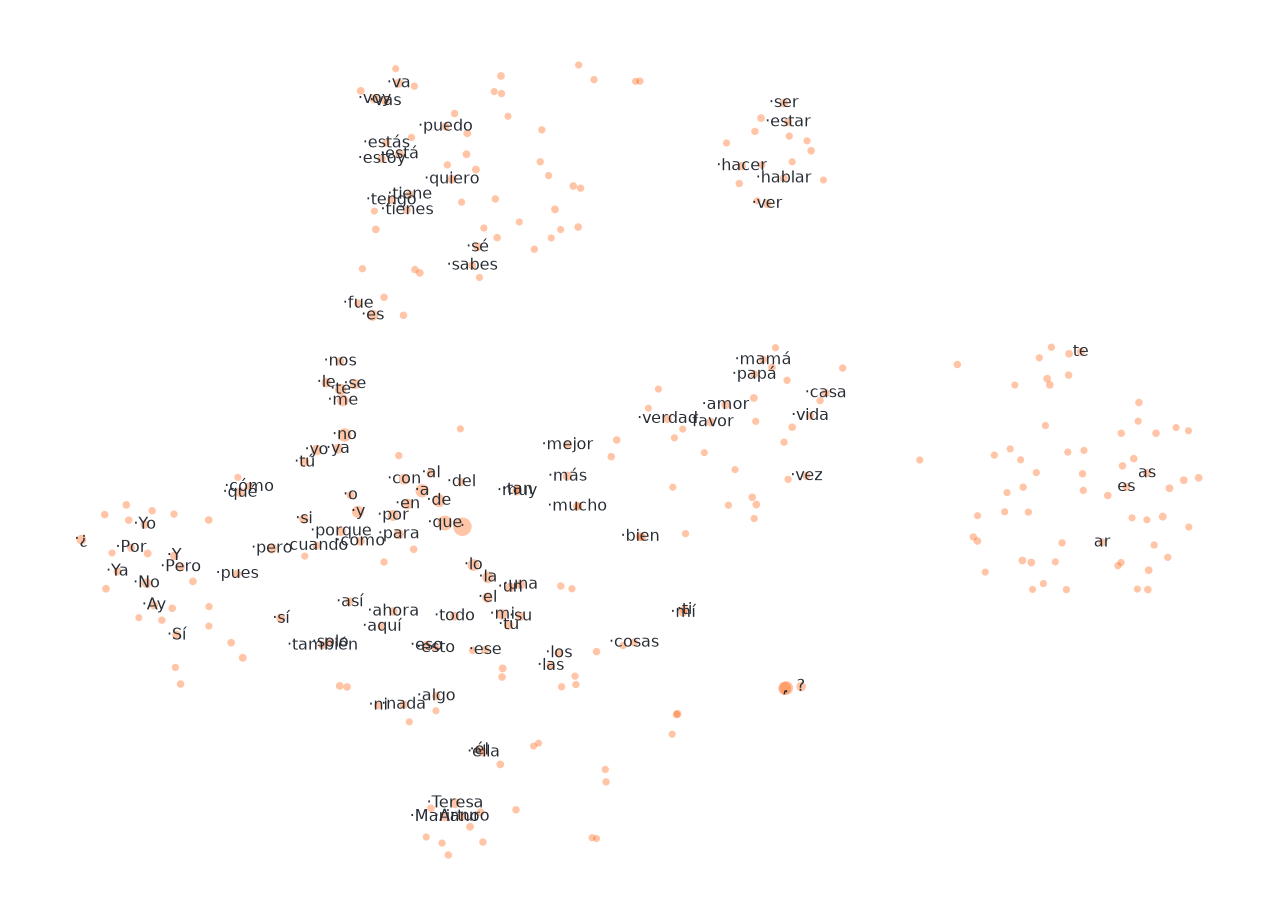
\includegraphics[width=0.88\textwidth]{embeddings.png}
\caption{Embeddings de token aprendidos por el mini GPT, proyectados a 2D con t-SNE (el punto \texttt{·} marca el espacio inicial). Tokens que el modelo usa de forma intercambiable tienden a agruparse: pronombres, nombres de personajes, signos de puntuación.}
\label{fig:embeddings}
\end{figure}

\subsection{La posición también cuenta}

``Teresa ama a Mariano'' y ``Mariano ama a Teresa'' contienen los mismos tokens. Como veremos, la atención trata su entrada como un conjunto: si permutamos los tokens, sus salidas se permutan igual. Para que el modelo distinga el orden, sumamos a cada token un vector que depende de su posición $t$, tomado de una segunda tabla $W_P\in\R^{T_{\mathrm{max}}\times d}$:
\begin{equation}\label{eq:h0}
  h^{(0)}_t = W_E[x_t] + W_P[t], \qquad t = 1,\dots,T.
\end{equation}
GPT-2 y nuestro modelo aprenden $W_P$ como cualquier otro parámetro, con $T_{\mathrm{max}} = 256$. Hay alternativas fijas (las sinusoides del transformer original) o rotaciones aplicadas dentro de la atención (RoPE, usada en Llama); aquí basta con la versión aprendida.

\begin{nota}[Pesos atados]
La última capa del modelo convierte un vector de dimensión $d$ en $V$ puntuaciones, una por token. Esa matriz tiene la misma forma que $W_E$ transpuesta, y GPT-2 usa literalmente la misma: $\text{logits} = h\,W_E^\top$. Así un token ``se lee'' y ``se escribe'' con el mismo vector, y nos ahorramos $V d$ parámetros.
\end{nota}

\begin{ejercicio}
\begin{enumerate}[label=\alph*)]
  \item Calcula cuántos parámetros tienen $W_E$ y $W_P$ en nuestro modelo. ¿Qué porcentaje del total (\mgParametros) representan?
  \item Demuestra que si $P$ es una matriz de permutación de $T\times T$, entonces $\softmax(PQK^\top P^\top)PV = P\,\softmax(QK^\top)V$ (sin máscara). ¿Qué dice esto sobre la necesidad de \eqref{eq:h0}?
\end{enumerate}
\end{ejercicio}

% ===========================================================================
\section{Atención: cada token decide a quién escuchar}\label{sec:atencion}

Consideremos la frase \emph{``Mariano, no me dejes sola''}. Para predecir lo que sigue a \emph{sola}, al modelo le sirve recordar que quien habla es una mujer (por eso \emph{sola} y no \emph{solo}) y que se dirige a Mariano. La información útil está repartida en posiciones anteriores, y en otra frase estará en otras. La atención es el mecanismo que permite a cada posición \emph{buscar} en las anteriores y traer lo que le sirve.

\subsection{Consultas, claves y valores}

Cada posición $t$, con su vector $h_t\in\R^d$, produce tres vectores mediante tres matrices aprendidas $W_Q, W_K\in\R^{d\times d_k}$ y $W_V\in\R^{d\times d_v}$:
\[
  q_t = h_t W_Q \quad(\text{consulta}),\qquad k_t = h_t W_K \quad(\text{clave}),\qquad v_t = h_t W_V \quad(\text{valor}).
\]
La consulta describe lo que la posición $t$ busca; la clave describe lo que la posición $s$ ofrece para ser encontrada; el valor es el contenido que entrega si la eligen. La compatibilidad entre lo que $t$ busca y lo que $s$ ofrece se mide con el producto punto $q_t\cdot k_s$.

\begin{intuicion}
Piensa en una biblioteca. Llegas con una pregunta (consulta), recorres los lomos de los libros (claves) y te llevas a casa una mezcla del contenido (valores) de los libros cuyo lomo se parece más a tu pregunta. La atención es esa mezcla, con pesos que suman uno.
\end{intuicion}

\subsection{Derivación paso a paso}

\textbf{Paso 1: afinidades.} Para la posición $t$ calculamos una puntuación con cada posición $s$:
\[
  s_{ts} = q_t \cdot k_s = \sum_{i=1}^{d_k} q_{t,i}\,k_{s,i}.
\]
Apilando las consultas en filas de una matriz $Q\in\R^{T\times d_k}$ y las claves en $K\in\R^{T\times d_k}$, todas las afinidades a la vez forman la matriz $S = QK^\top \in\R^{T\times T}$.

\textbf{Paso 2: escalar.} Dividimos entre $\sqrt{d_k}$ (justificamos esto en la siguiente subsección):
\[
  \tilde S = \frac{QK^\top}{\sqrt{d_k}}.
\]

\textbf{Paso 3: convertir en pesos.} Queremos pesos positivos que sumen uno sobre $s$. La función softmax hace exactamente eso, fila por fila:
\begin{equation}\label{eq:softmax}
  a_{ts} = \softmax(\tilde S_{t,:})_s = \frac{\exp(\tilde s_{ts})}{\sum_{s'} \exp(\tilde s_{ts'})},\qquad a_{ts} > 0,\quad \sum_s a_{ts} = 1 .
\end{equation}

\textbf{Paso 4: mezclar los valores.} La salida de la posición $t$ es el promedio ponderado de los valores:
\[
  o_t = \sum_{s} a_{ts}\, v_s .
\]
En forma matricial, con $V\in\R^{T\times d_v}$ los valores apilados (aquí $V$ denota la matriz de valores, sin confusión con el tamaño de vocabulario por el contexto):

\begin{definicion}[Atención de producto punto escalado]
\[
  \operatorname{Atención}(Q, K, V) = \softmax\!\left(\frac{QK^\top}{\sqrt{d_k}}\right) V \;\in\; \R^{T\times d_v}.
\]
\end{definicion}

\begin{ejemplo}[Tres tokens, $d_k = 2$]
Sean las consultas y claves de \emph{``no me dejes''}:
\[
Q = \begin{pmatrix} 1 & 0\\ 0 & 1\\ 1 & 1\end{pmatrix},\qquad
K = \begin{pmatrix} 1 & 0\\ 1 & 1\\ 0 & 2\end{pmatrix},\qquad
V = \begin{pmatrix} 1 & 0\\ 0 & 1\\ 2 & 2\end{pmatrix}.
\]
Para la tercera posición (\emph{dejes}), $q_3 = (1,1)$ y las afinidades son $q_3\cdot k_1 = 1$, $q_3\cdot k_2 = 2$, $q_3\cdot k_3 = 2$. Escalando por $\sqrt 2\approx 1.414$ obtenemos $(0.707, 1.414, 1.414)$. Sus exponenciales son $(2.03, 4.11, 4.11)$, que suman $10.25$, de modo que
\[
  a_{3,:} = (0.198,\ 0.401,\ 0.401),\qquad o_3 = 0.198\,(1,0) + 0.401\,(0,1) + 0.401\,(2,2) = (1.00,\ 1.20).
\]
La tercera posición atiende casi por igual a \emph{me} y a sí misma, y poco a \emph{no}.
\end{ejemplo}

\subsection{¿Por qué dividir entre $\sqrt{d_k}$?}

Supongamos que, al inicio del entrenamiento, las componentes de $q$ y de $k$ son variables aleatorias independientes con media $0$ y varianza $1$. Calculemos la media y la varianza del producto punto.

\begin{teorema}[Varianza del producto punto]
Si $q_i, k_i$, $i = 1,\dots,d_k$, son independientes con $\E[q_i]=\E[k_i]=0$ y $\operatorname{Var}(q_i)=\operatorname{Var}(k_i)=1$, entonces
\[
  \E[q\cdot k] = 0, \qquad \operatorname{Var}(q\cdot k) = d_k, \qquad \operatorname{Var}\!\left(\frac{q\cdot k}{\sqrt{d_k}}\right) = 1 .
\]
\end{teorema}

\textit{Demostración.} Por linealidad de la esperanza y la independencia, $\E[q_i k_i] = \E[q_i]\,\E[k_i] = 0$, así que $\E[q\cdot k] = 0$. Para la varianza, cada término cumple
\[
  \operatorname{Var}(q_i k_i) = \E[q_i^2 k_i^2] - \big(\E[q_i k_i]\big)^2 = \E[q_i^2]\,\E[k_i^2] - 0 = 1\cdot 1 = 1 .
\]
Los términos $q_i k_i$ son independientes entre sí, de modo que las varianzas se suman: $\operatorname{Var}(q\cdot k) = \sum_{i=1}^{d_k} 1 = d_k$. Finalmente, $\operatorname{Var}(cX) = c^2\operatorname{Var}(X)$ con $c = 1/\sqrt{d_k}$ da $d_k/d_k = 1$. $\square$

¿Qué pasa si no escalamos? Con $d_k = 64$ las afinidades tendrían desviación estándar $8$: diferencias de $20$ o $30$ entre posiciones serían comunes. El softmax de números así de separados es prácticamente un vector \emph{one-hot}. Eso es grave porque la derivada del softmax es
\begin{equation}\label{eq:jacobiano}
  \frac{\partial a_{t s}}{\partial \tilde s_{t r}} = a_{ts}\,\big(\delta_{sr} - a_{tr}\big),
\end{equation}
y si un peso vale casi $1$ y los demás casi $0$, todos estos términos son casi cero: el gradiente no fluye y la atención no aprende. Dividir entre $\sqrt{d_k}$ mantiene las afinidades en una escala donde el softmax todavía está ``blando''.

\begin{figure}[H]
\centering
\begin{tikzpicture}
\begin{axis}[width=0.62\textwidth, height=4.4cm, xlabel={$d_k$}, ylabel={desv. estándar}, xmode=log, log basis x=2,
  xtick={4,16,64,256}, xticklabels={4,16,64,256}, ymin=0, ymax=17, grid=major, grid style={gray!20},
  legend style={draw=none, font=\scriptsize, at={(0.02,0.98)}, anchor=north west}, tick label style={font=\scriptsize}, label style={font=\small}]
\addplot[very thick, color=pizarra, domain=2:256, samples=40] {sqrt(x)};
\addlegendentry{$q\cdot k$ sin escalar: $\sqrt{d_k}$}
\addplot[very thick, color=anahuac, domain=2:256, samples=2] {1};
\addlegendentry{$q\cdot k/\sqrt{d_k}$: siempre 1}
\end{axis}
\end{tikzpicture}
\caption{La escala de las afinidades crece como $\sqrt{d_k}$ si no se corrige.}
\label{fig:varianza}
\end{figure}

\subsection{La máscara causal}

Durante el entrenamiento le mostramos al modelo una ventana completa de texto y le pedimos predecir, en cada posición, el token siguiente. Si la posición $t$ pudiera atender a la posición $t+1$, simplemente copiaría la respuesta. Para impedirlo sumamos una matriz $M$ antes del softmax:
\begin{equation}\label{eq:mascara}
  \operatorname{AtenciónCausal}(Q,K,V) = \softmax\!\left(\frac{QK^\top}{\sqrt{d_k}} + M\right)V,\qquad
  M_{ts} = \begin{cases} 0 & \text{si } s \le t,\\ -\infty & \text{si } s > t. \end{cases}
\end{equation}
Como $e^{-\infty} = 0$, los pesos hacia el futuro son exactamente cero y cada fila sigue sumando uno sobre las posiciones permitidas. La matriz de pesos queda triangular inferior (figura~\ref{fig:mascara}).

\begin{figure}[H]
\centering
\begin{tikzpicture}[scale=0.62]
\foreach \w [count=\n] in {Mariano,no,me,dejes,sola} {
  \pgfmathtruncatemacro{\i}{\n-1}
  \foreach \j in {0,...,4} {
    \ifnum\j>\i
      \fill[grisclaro] (\j,-\i) rectangle ++(1,-1);
      \node[font=\scriptsize, text=gray] at (\j+0.5,-\i-0.5) {$-\infty$};
    \else
      \pgfmathsetmacro{\op}{1/(\i+1)}
      \fill[anahuac, opacity=\op] (\j,-\i) rectangle ++(1,-1);
    \fi
    \draw[white, thick] (\j,-\i) rectangle ++(1,-1);
  }
  \node[anchor=east, font=\footnotesize\ttfamily] at (-0.1,-\i-0.5) {\w};
  \node[anchor=south west, rotate=45, font=\footnotesize\ttfamily] at (\i+0.3,0.05) {\w};
}
\node[font=\small\sffamily, rotate=90] at (-3.4,-2.5) {consulta (posición $t$)};
\node[font=\small\sffamily] at (2.5,2.6) {clave (posición $s$)};
\end{tikzpicture}
\caption{Máscara causal. Cada fila es una posición que pregunta; solo puede repartir su atención (naranja) entre ella misma y las posiciones anteriores. Aquí se dibuja el caso de atención uniforme, $a_{ts} = 1/t$.}
\label{fig:mascara}
\end{figure}

\begin{nota}
Gracias a la máscara, una sola pasada hacia adelante sobre una ventana de $T$ tokens produce $T$ ejemplos de entrenamiento a la vez: la posición 1 predice el token 2, la posición 2 predice el token 3, y así sucesivamente, cada una sin hacer trampa.
\end{nota}

\begin{ejercicio}
\begin{enumerate}[label=\alph*)]
  \item Repite el ejemplo de tres tokens para la segunda posición, aplicando la máscara causal. ¿Cuánto valen $a_{2,:}$ y $o_2$?
  \item Verifica la fórmula~\eqref{eq:jacobiano} derivando~\eqref{eq:softmax}. Evalúala en $a = (0.98, 0.01, 0.01)$ y en $a = (1/3, 1/3, 1/3)$. ¿En cuál caso el gradiente es más grande?
  \item Si las componentes de $q$ y $k$ tuvieran varianza $\sigma^2$ en lugar de $1$, ¿por cuánto habría que dividir $q\cdot k$ para que su varianza fuera $1$?
  \item Explica qué aprendería un modelo entrenado sin máscara y por qué fallaría al generar texto.
\end{enumerate}
\end{ejercicio}

% ===========================================================================
\section{Atención multi-cabeza}\label{sec:multi}

Una sola atención produce un único patrón de pesos por posición. Pero al leer \emph{``Juro que me las vas a pagar''} hay varias relaciones simultáneas: la concordancia entre \emph{vas} y su sujeto implícito, la palabra inmediatamente anterior, el verbo que abre la frase. La solución es tener varias atenciones en paralelo, llamadas \textbf{cabezas}, cada una con sus propias proyecciones.

\begin{definicion}[Atención multi-cabeza]
Con $H$ cabezas y $d_k = d_v = d/H$, la cabeza $j$ tiene sus matrices $W_Q^{(j)}, W_K^{(j)}, W_V^{(j)}\in\R^{d\times d_k}$ y calcula
\[
  \text{cabeza}_j = \operatorname{AtenciónCausal}\big(XW_Q^{(j)},\, XW_K^{(j)},\, XW_V^{(j)}\big)\in\R^{T\times d_k}.
\]
Las salidas se concatenan y se mezclan con una proyección $W_O\in\R^{d\times d}$:
\[
  \operatorname{MHA}(X) = \big[\text{cabeza}_1;\ \text{cabeza}_2;\ \dots;\ \text{cabeza}_H\big]\,W_O \in \R^{T\times d}.
\]
\end{definicion}

En nuestro modelo $d = 384$ y $H = 6$, así que cada cabeza trabaja en $d_k = 64$ dimensiones. El costo total es el mismo que el de una sola cabeza de dimensión $384$: repartimos la capacidad en seis ``puntos de vista''. En el código, las tres proyecciones de todas las cabezas viven en una sola matriz de $d\times 3d$ y el tensor se reacomoda con \texttt{view} y \texttt{transpose} para obtener la forma $(B, H, T, d_k)$.

\begin{lstlisting}[language=Python, caption={Atención causal multi-cabeza, tal como está en \texttt{scripts/train\_minigpt\_teresa.py}.}]
q, k, v = self.qkv(x).split(C, dim=2)              # (B, T, C) cada una
d_k = C // self.n_head
q, k, v = (t.view(B, T, self.n_head, d_k).transpose(1, 2) for t in (q, k, v))
s = (q @ k.transpose(-2, -1)) / math.sqrt(d_k)       # (B, H, T, T)
s = s.masked_fill(~self.mascara[:T, :T], float("-inf"))
a = F.softmax(s, dim=-1)                             # pesos de atención
y = (a @ v).transpose(1, 2).contiguous().view(B, T, C)   # concatenar cabezas
return self.proy(y)                                  # W_O
\end{lstlisting}

La figura~\ref{fig:cabezas} muestra las seis cabezas de la primera y de la última capa del modelo entrenado sobre la frase \emph{``Teresa, yo te amo con toda mi alma''}. En la primera capa casi todas las cabezas miran sobre todo al propio token y a sus vecinos inmediatos. En la última capa ya hay especialistas: la cabeza 2 mira casi siempre al token anterior (una diagonal justo debajo de la principal), la cabeza 1 descansa en el primer token (una columna intensa a la izquierda, que funciona como lugar de descanso cuando no hay nada útil que mirar) y en la cabeza 4 las palabras que siguen a \emph{amo} vuelven a mirar a ese verbo.

\begin{figure}[H]
\centering
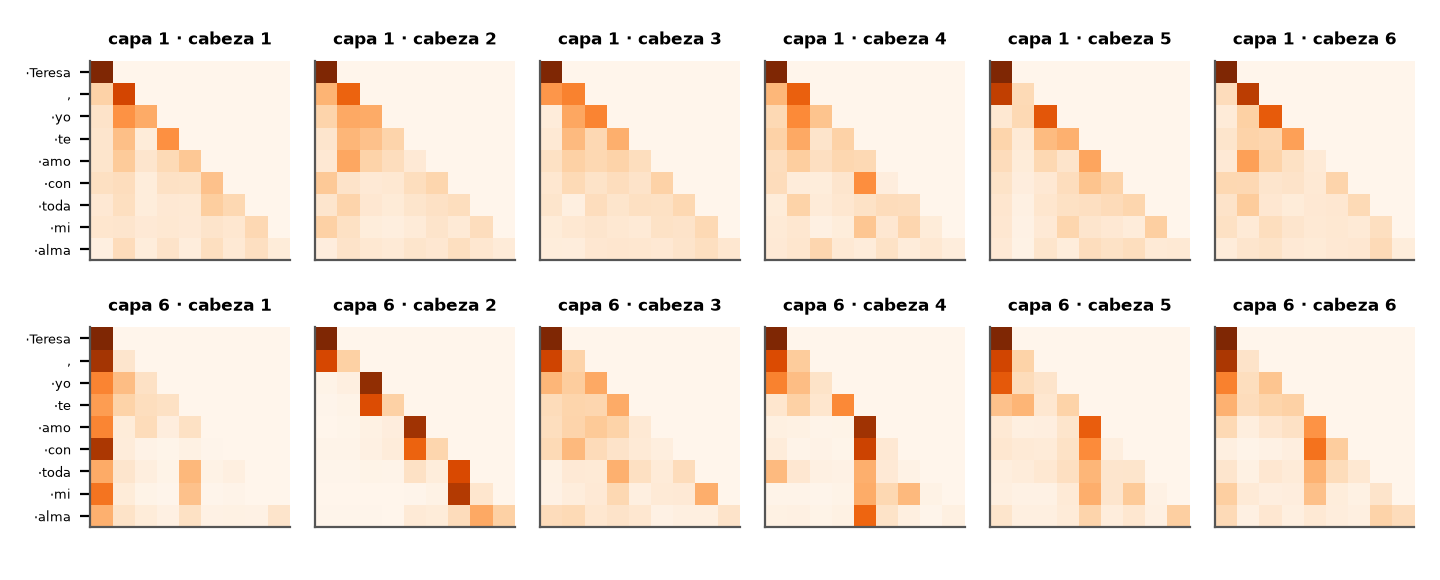
\includegraphics[width=\textwidth]{atencion_cabezas.png}
\caption{Pesos de atención reales del mini GPT entrenado. Fila superior: capa 1; fila inferior: capa 6. En cada panel, la fila es la posición que pregunta y la columna la que responde. El triángulo superior está vacío por la máscara causal.}
\label{fig:cabezas}
\end{figure}

\begin{figure}[H]
\centering
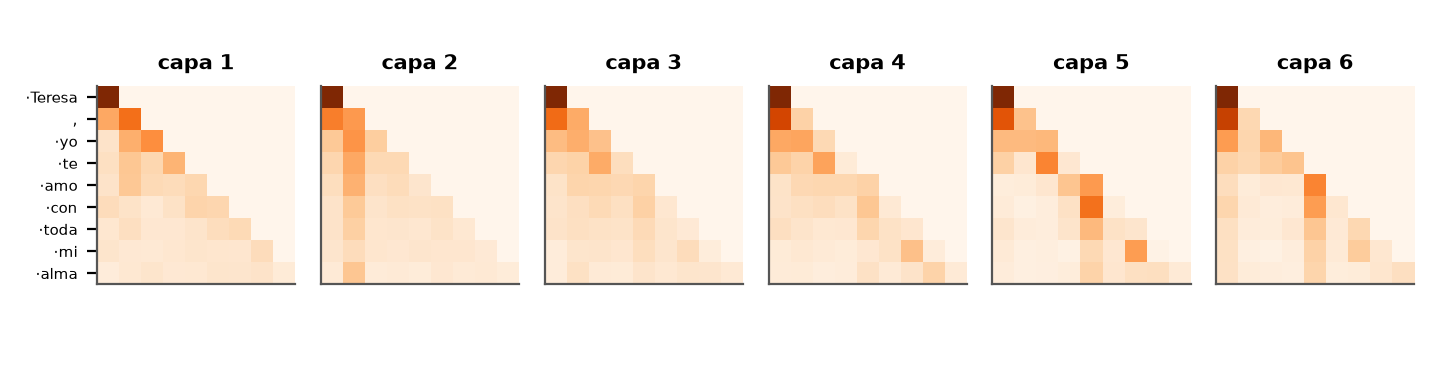
\includegraphics[width=\textwidth]{atencion_capas.png}
\caption{Promedio de las seis cabezas en cada una de las seis capas, para la misma frase.}
\label{fig:capas}
\end{figure}

\begin{ejercicio}
\begin{enumerate}[label=\alph*)]
  \item Cuenta los parámetros de la atención multi-cabeza (con sesgos) en función de $d$. Verifica que no dependen de $H$.
  \item La matriz de pesos de atención de una capa tiene forma $(B, H, T, T)$. Con $B = 32$, $H = 6$, $T = 256$ y números de 2 bytes, ¿cuánta memoria ocupa por capa? ¿Y con $T = 4096$?
  \item En la figura~\ref{fig:cabezas}, identifica una cabeza que mire principalmente al token anterior. ¿Para qué le serviría eso al modelo?
\end{enumerate}
\end{ejercicio}

% ===========================================================================
\section{El bloque transformer}\label{sec:bloque}

La atención mezcla información \emph{entre} posiciones. Para procesar la información \emph{dentro} de cada posición, el bloque agrega una red feed-forward, y para que la pila de bloques se pueda entrenar con muchas capas usa dos ingredientes más: normalización y conexiones residuales.

\subsection{LayerNorm}

\begin{definicion}[Normalización por capa]
Para un vector $x\in\R^d$,
\[
  \mu = \frac1d\sum_{i=1}^d x_i,\qquad \sigma^2 = \frac1d\sum_{i=1}^d (x_i-\mu)^2,\qquad
  \operatorname{LN}(x)_i = \gamma_i\,\frac{x_i - \mu}{\sqrt{\sigma^2 + \varepsilon}} + \beta_i ,
\]
con $\gamma,\beta\in\R^d$ aprendidos y $\varepsilon$ pequeño (por ejemplo $10^{-5}$) para evitar dividir entre cero.
\end{definicion}

LayerNorm normaliza cada token por separado, sin mirar al resto del lote. Eso mantiene la escala de las activaciones estable de capa en capa, de modo que las afinidades de la atención no exploten ni se apaguen.

\subsection{La red feed-forward}

\begin{definicion}[FFN]
A cada posición se le aplica la misma red de dos capas con expansión $4d$:
\[
  \operatorname{FFN}(x) = \operatorname{GELU}(xW_1 + b_1)\,W_2 + b_2,\qquad W_1\in\R^{d\times 4d},\ W_2\in\R^{4d\times d},
\]
donde $\operatorname{GELU}(u) = u\,\Phi(u) \approx \tfrac12 u\big(1+\tanh\!\big[\sqrt{2/\pi}\,(u + 0.044715\,u^3)\big]\big)$ y $\Phi$ es la distribución acumulada normal estándar.
\end{definicion}

Si la atención es la conversación entre tokens, la FFN es el momento en que cada token ``piensa'' a solas con lo que escuchó. Dos tercios de los parámetros de cada bloque están aquí.

\subsection{Conexiones residuales y el bloque completo}

\begin{definicion}[Bloque pre-LN, estilo GPT-2]
\begin{align*}
  x' &= x + \operatorname{MHA}\big(\operatorname{LN}_1(x)\big),\\
  x'' &= x' + \operatorname{FFN}\big(\operatorname{LN}_2(x')\big).
\end{align*}
\end{definicion}

La suma $x + f(x)$ se llama \textbf{conexión residual}. Su derivada respecto de $x$ es $I + \partial f/\partial x$: aunque $\partial f/\partial x$ sea pequeña, el término identidad garantiza que el gradiente llegue intacto a las capas de abajo. Conviene imaginar un ``flujo residual'' que recorre el modelo de abajo arriba, al que cada subcapa le suma una pequeña corrección.

\begin{figure}[H]
\centering
\begin{tikzpicture}[
  caja/.style={draw=pizarra, rounded corners=2pt, minimum width=34mm, minimum height=7mm, font=\sffamily\small, fill=white},
  ln/.style={caja, fill=grisclaro},
  atn/.style={caja, fill=naranjabg, draw=anahuac},
  ffn/.style={caja, fill=azuldefbg, draw=azuldef},
  suma/.style={circle, draw=pizarra, inner sep=0pt, minimum size=5mm, font=\small},
  f/.style={-Stealth, thick, pizarra}]
\node (in) at (0,0) {$x$};
\node[ln] (ln1) at (0,1.2) {LayerNorm};
\node[atn] (mha) at (0,2.3) {Atención multi-cabeza};
\node[suma] (s1) at (0,3.4) {$+$};
\node[ln] (ln2) at (0,4.5) {LayerNorm};
\node[ffn] (ffn) at (0,5.6) {FFN ($d\to 4d\to d$)};
\node[suma] (s2) at (0,6.7) {$+$};
\node (out) at (0,7.7) {$x''$};
\draw[f] (in) -- (ln1); \draw[f] (ln1) -- (mha); \draw[f] (mha) -- (s1);
\draw[f] (s1) -- (ln2); \draw[f] (ln2) -- (ffn); \draw[f] (ffn) -- (s2); \draw[f] (s2) -- (out);
\draw[f, anahuac] (0,0.45) -- (-2.4,0.45) |- (s1.west);
\draw[f, anahuac] (0,3.85) -- (-2.4,3.85) |- (s2.west);
\node[font=\scriptsize\sffamily, text=anahuac, rotate=90] at (-2.7,2) {residual};
\node[font=\scriptsize\sffamily, text=anahuac, rotate=90] at (-2.7,5.3) {residual};
\node[font=\footnotesize, anchor=west, text width=6.4cm] at (2.3,2.3) {$\softmax\!\big(\frac{QK^\top}{\sqrt{d_k}}+M\big)V$ por cabeza, luego $[\cdot]\,W_O$};
\node[font=\footnotesize, anchor=west, text width=6.4cm] at (2.3,5.6) {$\operatorname{GELU}(xW_1+b_1)W_2+b_2$};
\node[font=\footnotesize, anchor=west, text width=6.4cm] at (2.3,1.2) {$\gamma\odot\frac{x-\mu}{\sigma}+\beta$};
\draw[decorate, decoration={brace, amplitude=6pt}, gray] (-3.1,0.2) -- (-3.1,7.2) node[midway, left=8pt, font=\sffamily\small, text=pizarra] {$\times 6$};
\end{tikzpicture}
\caption{Un bloque transformer pre-LN. El modelo apila seis bloques idénticos (con pesos distintos) y termina con un LayerNorm final y la capa de salida atada a los embeddings.}
\label{fig:bloque}
\end{figure}

\subsection{Cuántos parámetros hay}

Contemos los parámetros de un bloque con dimensión $d$:
\begin{itemize}
  \item Atención: $W_Q, W_K, W_V$ y sus sesgos dan $3d^2 + 3d$; la proyección $W_O$ con su sesgo, $d^2 + d$. Total $4d^2 + 4d$.
  \item FFN: $W_1$ y $b_1$ dan $4d^2 + 4d$; $W_2$ y $b_2$ dan $4d^2 + d$. Total $8d^2 + 5d$.
  \item Dos LayerNorm: $2\cdot 2d = 4d$.
\end{itemize}
En total, $12d^2 + 13d$ por bloque. Con $d = 384$ son $1\,774\,464$ parámetros por bloque y $10\,646\,784$ en los seis. Sumando $W_E$ ($\mgVocab\times 384$), $W_P$ ($256\times 384$) y el LayerNorm final, el modelo tiene \mgParametros{} parámetros, unos \mgParametrosM{} millones. GPT-2 pequeño tiene 124 millones; GPT-3, 175 mil millones.

\begin{table}[H]
\centering
\begin{tabular}{@{}lr@{}}
\toprule
Hiperparámetro & Valor \\
\midrule
Capas $N$ & 6 \\
Dimensión $d$ & 384 \\
Cabezas $H$ (con $d_k = 64$) & 6 \\
Contexto $T_{\mathrm{max}}$ & 256 tokens \\
Vocabulario $V$ (SentencePiece BPE) & \mgVocab \\
Dropout & 0.2 \\
Parámetros & \mgParametros \\
\bottomrule
\end{tabular}
\caption{Configuración del mini GPT de la sesión.}
\label{tab:config}
\end{table}

\begin{ejercicio}
\begin{enumerate}[label=\alph*)]
  \item Verifica el conteo $12d^2 + 13d$ con $d = 768$ y compara con los 7.1 millones por bloque de GPT-2 pequeño.
  \item Calcula $\operatorname{LN}(x)$ para $x = (2, 4, 6)$ con $\gamma = (1,1,1)$, $\beta = 0$ y $\varepsilon = 0$.
  \item El transformer original usaba post-LN: $x' = \operatorname{LN}(x + \operatorname{MHA}(x))$. Argumenta, con la derivada de la conexión residual, por qué pre-LN facilita entrenar muchas capas.
\end{enumerate}
\end{ejercicio}

% ===========================================================================
\section{Entrenamiento}\label{sec:entrenamiento}

\subsection{Entropía cruzada y perplejidad}

Para cada posición, el modelo produce un vector de \emph{logits} $z\in\R^V$ y, con softmax, una distribución $p = \softmax(z)$. Si el token correcto es $y$, la pérdida en esa posición es el logaritmo negativo de la probabilidad que el modelo le dio:
\begin{equation}\label{eq:ce}
  \ell = -\log p_y = -z_y + \log\sum_{j=1}^{V} e^{z_j}.
\end{equation}
Promediando sobre las $B$ secuencias del lote y las $T$ posiciones de cada una:
\[
  \mathcal{L}(\theta) = -\frac{1}{BT}\sum_{b=1}^{B}\sum_{t=1}^{T} \log p_\theta\big(x_{b,t+1}\mid x_{b,\le t}\big).
\]
Derivando \eqref{eq:ce} respecto del logit $z_j$ aparece un resultado sorprendentemente sencillo:
\[
  \frac{\partial \ell}{\partial z_j} = -\mathbf{1}[j = y] + \frac{e^{z_j}}{\sum_k e^{z_k}} = p_j - \mathbf{1}[j=y].
\]
El gradiente es la diferencia entre lo que el modelo predijo y lo que debió predecir: empuja hacia arriba el logit correcto y hacia abajo los demás, en proporción a su probabilidad.

\begin{definicion}[Perplejidad]
\[
  \operatorname{PPL} = \exp(\mathcal{L}).
\]
Se interpreta como el número efectivo de opciones entre las que el modelo duda en cada paso. Un modelo que reparte uniformemente entre $V$ tokens tiene $\mathcal{L} = \ln V$ y $\operatorname{PPL} = V$.
\end{definicion}

Con $V = \mgVocab$, la pérdida de un modelo recién inicializado debe rondar $\ln \mgVocab = \mgLnV$. Es la primera comprobación que conviene hacer antes de entrenar.

\subsection{AdamW}

El descenso de gradiente simple, $\theta \leftarrow \theta - \eta\,g$, usa el mismo tamaño de paso para todos los parámetros. Adam (Kingma y Ba, 2015) adapta el paso de cada parámetro con promedios móviles del gradiente y de su cuadrado. AdamW (Loshchilov y Hutter, 2019) además separa el decaimiento de pesos del gradiente.

\begin{definicion}[AdamW]
Con gradiente $g_t$, tasa $\eta_t$, coeficientes $\beta_1, \beta_2$ y decaimiento $\lambda$:
\begin{align*}
  m_t &= \beta_1 m_{t-1} + (1-\beta_1)\, g_t, & \hat m_t &= \frac{m_t}{1-\beta_1^t},\\
  v_t &= \beta_2 v_{t-1} + (1-\beta_2)\, g_t^2, & \hat v_t &= \frac{v_t}{1-\beta_2^t},\\
  \theta_t &= \theta_{t-1} - \eta_t\left(\frac{\hat m_t}{\sqrt{\hat v_t} + \varepsilon} + \lambda\,\theta_{t-1}\right).
\end{align*}
\end{definicion}

El cociente $\hat m_t/\sqrt{\hat v_t}$ tiene magnitud cercana a 1 para todos los parámetros, así que $\eta_t$ fija directamente el tamaño típico del paso. El término $\lambda\theta$ encoge los pesos hacia cero y actúa como regularización. Usamos $\beta_1 = 0.9$, $\beta_2 = 0.95$ y $\lambda = 0.1$, aplicado solo a las matrices (los sesgos y los parámetros de LayerNorm no se encogen).

\subsection{Calendario de la tasa de aprendizaje}

Al inicio los momentos $m$ y $v$ son ruidosos y un paso grande puede desestabilizar el modelo. Por eso la tasa sube linealmente durante $W$ pasos de \emph{calentamiento} y luego baja suavemente siguiendo medio periodo de coseno hasta $\eta_{\mathrm{min}}$ en el paso final $S$:
\begin{equation}\label{eq:coseno}
  \eta_t = \begin{cases}
    \eta_{\mathrm{max}}\,\dfrac{t}{W}, & t < W,\\[2mm]
    \eta_{\mathrm{min}} + \dfrac12\big(\eta_{\mathrm{max}}-\eta_{\mathrm{min}}\big)\left(1 + \cos\!\left(\pi\,\dfrac{t - W}{S - W}\right)\right), & W \le t \le S.
  \end{cases}
\end{equation}

\begin{figure}[H]
\centering
\begin{tikzpicture}
\begin{axis}[width=0.75\textwidth, height=4cm, xlabel={paso $t$}, ylabel={$\eta_t$ ($\times10^{-4}$)}, xmin=0, xmax=6000, ymin=0, ymax=6.8,
  grid=major, grid style={gray!20}, tick label style={font=\scriptsize}, label style={font=\small}, scaled x ticks=false]
\addplot[very thick, anahuac, domain=0:300, samples=2] {6*x/300};
\addplot[very thick, anahuac, domain=300:6000, samples=80] {0.6 + 0.5*(6-0.6)*(1+cos(deg(pi*(x-300)/5700)))};
\draw[dashed, gray] (axis cs:300,0) -- (axis cs:300,6.5) node[above, font=\scriptsize] {$W$};
\end{axis}
\end{tikzpicture}
\caption{Calendario \eqref{eq:coseno} con $\eta_{\mathrm{max}} = 6\times10^{-4}$, $\eta_{\mathrm{min}} = \eta_{\mathrm{max}}/10$, $W = 300$ y $S = 6000$.}
\label{fig:coseno}
\end{figure}

\subsection{Recorte del gradiente}

De vez en cuando un lote produce un gradiente enorme. Para que un solo lote no arruine el entrenamiento, si la norma del gradiente completo supera un umbral $c$ se reescala:
\[
  g \leftarrow g\cdot\min\!\left(1,\ \frac{c}{\norm{g}_2}\right),\qquad c = 1.
\]
La dirección se conserva; solo se limita la longitud del paso.

\subsection{Lo que pasó en la RTX 3070}

Entrenamos con lotes de 32 ventanas de 256 tokens ($8\,192$ tokens por paso), precisión mixta \texttt{bfloat16}, dropout de 0.2 y evaluación cada 250 pasos sobre \mgCapitulosVal{} capítulos completos reservados para validación. El entrenamiento se detiene si la pérdida de validación deja de mejorar durante varias evaluaciones seguidas, y se conserva el checkpoint con la menor pérdida de validación. Se corrieron \mgPasos{} pasos en \mgMinutos{} minutos, con un pico de \mgVRAM{}~GB de memoria de video.

\begin{figure}[H]
\centering
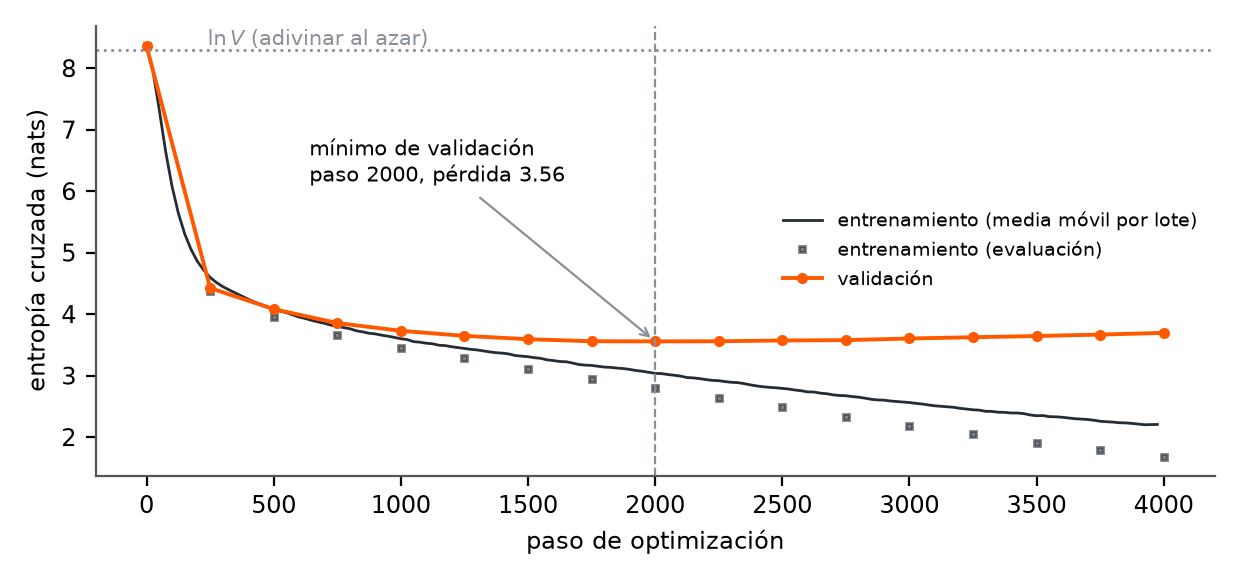
\includegraphics[width=0.92\textwidth]{curva_perdida.png}
\caption{Curvas reales de pérdida. La validación alcanza su mínimo, \mgMejorVal{} nats (perplejidad \mgMejorPPL), en el paso \mgMejorPaso, tras unas \mgEpocasMejor{} pasadas por el corpus. Después, el entrenamiento sigue bajando mientras la validación sube: el modelo empieza a memorizar. Los cuadros grises se evalúan sin dropout y por eso quedan debajo de la media móvil, que se mide con dropout activo.}
\label{fig:curva}
\end{figure}

La figura~\ref{fig:curva} cuenta la historia completa. Al principio ambas curvas caen juntas desde $\ln V$: el modelo aprende qué tokens son frecuentes, luego qué sílabas van juntas, luego frases hechas. Llega un punto en que la curva de entrenamiento se separa de la de validación. Con apenas \mgCorpusMB{}~MB de texto y \mgParametrosM{} millones de parámetros, el modelo tiene capacidad de sobra para memorizar capítulos, y eso mejora la pérdida en los capítulos que ve sin ayudar en los que no ve. Por eso guardamos el checkpoint del mínimo de validación.

\begin{intuicion}
Una perplejidad de \mgMejorPPL{} quiere decir que, en promedio, el modelo duda entre unas \mgMejorPPL{} piezas para cada siguiente token. Parece mucho, pero hay que compararlo con las \mgVocab{} opciones de partida: el modelo descartó en cada paso alrededor del \mgDescartado\,\% del vocabulario.
\end{intuicion}

\begin{ejercicio}
\begin{enumerate}[label=\alph*)]
  \item Demuestra que $\partial\ell/\partial z_j = p_j - \mathbf{1}[j=y]$ a partir de \eqref{eq:ce}.
  \item ¿Cuánto vale la tasa \eqref{eq:coseno} en $t = W$, en el punto medio entre $W$ y $S$, y en $t = S$?
  \item Si la pérdida de validación es $3.9$, ¿cuál es la perplejidad? ¿Y si baja a $3.5$? Expresa la mejora como porcentaje de perplejidad.
  \item Propón dos cambios para retrasar el sobreajuste sin conseguir más datos y explica por qué funcionarían.
\end{enumerate}
\end{ejercicio}

% ===========================================================================
\section{Generación de texto}\label{sec:generacion}

Con el modelo entrenado, generar es un bucle: calcular la distribución del siguiente token, elegir uno, agregarlo al contexto y repetir. La parte interesante es \emph{cómo elegir}.

\subsection{Temperatura}

\begin{definicion}[Softmax con temperatura]
Dados los logits $z$ y una temperatura $\tau > 0$,
\[
  p_i(\tau) = \frac{\exp(z_i/\tau)}{\sum_{j}\exp(z_j/\tau)} .
\]
\end{definicion}
Con $\tau = 1$ recuperamos la distribución del modelo. Si $\tau\to 0$, el término con el mayor logit domina y la distribución se concentra en un solo token: es la \emph{búsqueda voraz}. Si $\tau\to\infty$, todos los $z_i/\tau$ tienden a $0$ y la distribución se vuelve uniforme. La figura~\ref{fig:temperatura} muestra el efecto sobre la distribución real que nuestro modelo asigna después de \emph{``yo te''}.

\begin{figure}[H]
\centering
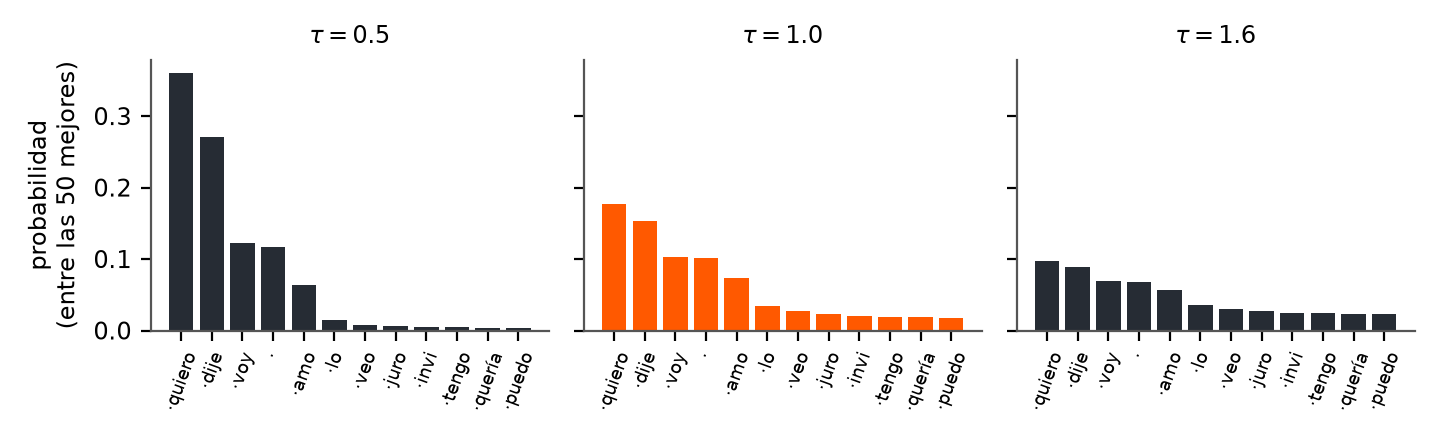
\includegraphics[width=\textwidth]{temperatura.png}
\caption{Distribución del siguiente token después de \emph{``yo te''} según el mini GPT, con tres temperaturas. A temperatura baja casi toda la masa se va a las primeras opciones; a temperatura alta la cola gana peso.}
\label{fig:temperatura}
\end{figure}

\subsection{Top-k y top-p}

Incluso con buena temperatura, la cola de miles de tokens improbables suma una masa considerable, y de vez en cuando el muestreo elige uno absurdo. Dos recortes lo evitan.

\begin{definicion}[Muestreo top-k]
Sea $S_k$ el conjunto de los $k$ tokens con mayor probabilidad. Se muestrea de
\[
  \tilde p_i = \frac{p_i\,\mathbf{1}[i\in S_k]}{\sum_{j\in S_k} p_j} .
\]
\end{definicion}

\begin{definicion}[Muestreo top-p o de núcleo]
Ordenamos las probabilidades de mayor a menor, $p_{(1)}\ge p_{(2)}\ge\cdots$, y tomamos el menor $m$ tal que
\[
  \sum_{i=1}^{m} p_{(i)} \ge p .
\]
El núcleo $S_p$ son esos $m$ tokens, y se renormaliza sobre ellos igual que en top-k (Holtzman et al., 2020).
\end{definicion}

La ventaja de top-p es que el tamaño del núcleo se adapta: después de \emph{``Arturo de la''} el modelo está casi seguro de \emph{``Barrera''} y el núcleo tiene uno o dos tokens; después de \emph{``yo te''} hay muchas continuaciones razonables y el núcleo crece.

\begin{ejemplo}[Núcleo a mano]
Supongamos que tras \emph{``yo te''} las cinco opciones más probables son \emph{quiero} (0.30), \emph{amo} (0.22), \emph{lo} (0.15), \emph{juro} (0.10) y \emph{dije} (0.06), y el resto suma 0.17. Con $p = 0.6$ las acumuladas son $0.30, 0.52, 0.67$: el núcleo es \{\emph{quiero}, \emph{amo}, \emph{lo}\} y, al renormalizar entre $0.67$, quedan $0.448$, $0.328$ y $0.224$. Con top-k y $k = 2$ el conjunto sería \{\emph{quiero}, \emph{amo}\} con $0.577$ y $0.423$.
\end{ejemplo}

\subsection{Cómo aprendió a hablar}

Generamos texto con el mismo comienzo (\emph{``Teresa, eres una''}), la misma semilla aleatoria, $\tau = 0.8$ y top-k $= 50$ en distintos momentos del entrenamiento. Las muestras son reales, sin editar:

\lstinputlisting[language={},numbers=none,basicstyle=\ttfamily\scriptsize,breaklines=true]{muestras.txt}

En el paso 0 el modelo produce piezas al azar. Pronto aprende qué piezas son frecuentes y dónde van los espacios; luego palabras completas, signos de puntuación y nombres de personajes; al final, frases con la gramática y el tono de un reclamo de telenovela. La gramática y el tono salieron por sí solos de minimizar la entropía cruzada.

\begin{nota}[Lo que no cubrimos]
Los modelos de producción agregan optimizaciones que no cambian las ideas de esta sesión. Al generar, guardan las claves y valores de los tokens anteriores para no recalcularlos (\emph{KV cache}); calculan la atención por bloques sin escribir la matriz $T\times T$ completa en memoria (FlashAttention, que PyTorch usa por dentro en \texttt{scaled\_dot\_product\_attention}); y comparten claves y valores entre grupos de cabezas para ahorrar memoria (GQA). Las ecuaciones de fondo son las mismas que derivamos aquí.
\end{nota}

\begin{ejercicio}
\begin{enumerate}[label=\alph*)]
  \item Demuestra que $\lim_{\tau\to 0^+} p_i(\tau) = \mathbf{1}[i = \argmax_j z_j]$ cuando el máximo es único, y que $\lim_{\tau\to\infty} p_i(\tau) = 1/V$.
  \item En el ejemplo del núcleo, ¿qué conjunto se obtiene con $p = 0.9$? ¿Y con $p = 0.3$?
  \item La entropía de una distribución es $\mathcal{H}(p) = -\sum_i p_i\log p_i$. Argumenta por qué $\mathcal{H}(p(\tau))$ crece con $\tau$.
  \item Usa la SPA de la sesión (\texttt{spa/minigpt\_teresa.html}) para encontrar una combinación de temperatura y top-p que produzca texto coherente pero variado. Reporta tus valores y justifícalos.
\end{enumerate}
\end{ejercicio}

\section*{Materiales de la sesión}
\addcontentsline{toc}{section}{Materiales de la sesión}
\begin{itemize}
  \item \texttt{scripts/descargar\_teresa.py}: descarga y limpieza del corpus.
  \item \texttt{scripts/train\_minigpt\_teresa.py}: entrenamiento completo en el servidor GPU y exportación de resultados.
  \item \texttt{notebooks/06\_minigpt\_teresa.ipynb}: el mismo recorrido paso a paso, con BPE a mano y atención calculada a mano.
  \item \texttt{spa/minigpt\_teresa.html}: tokenizador en vivo, atención interactiva, laboratorio de muestreo y mapa de embeddings.
\end{itemize}

\textbf{Referencias.} Vaswani et al. (2017), \emph{Attention is all you need}. Radford et al. (2019), \emph{Language models are unsupervised multitask learners}. Sennrich, Haddow y Birch (2016), \emph{Neural machine translation of rare words with subword units}. Kudo y Richardson (2018), \emph{SentencePiece}. Loshchilov y Hutter (2019), \emph{Decoupled weight decay regularization}. Holtzman et al. (2020), \emph{The curious case of neural text degeneration}. Raschka (2024), \emph{Build a large language model (from scratch)}.

\end{document}
